\section{Sourdough bread}
\textit{Mostly rye-based sourdough bread}

\subsection*{Ingredients}

\textit{Rye flour (type 997) and just one type of plain white wheat flour work as well, although type 550 and 1050 give a nicer flavor than the normal type 405 flour.}

\textbf{for the sourdough}\\
\begin{tabular}{ l l }
  120g & rye flour (type 1150) \\
  20g & sourdough starter \\
  100ml & warm water (40$^\circ$C) \\
\end{tabular}

\textbf{for the soaker}\\
\begin{tabular}{ l l }
  30g & oatmeal \\
  30g & ground dried bread (just keep the dried leftovers from your last loaf of bread for this) \\
  100ml & boiling water\\
\end{tabular}

\textbf{for the dough}\\
\begin{tabular}{ l l }
 220g & rye flour (type 1150) \\
 120g & wheat flour (type 550) \\
 100g & wheat flour (type 1050) \\
 12-14g & salt \\
 10g & fresh yeast \\
 3g (or more) & finely ground coriander, fennel, and caraway seeds \\
 200ml & water (25$^\circ$C) \\
\end{tabular}

\subsection*{Description}
\begin{enumerate}
	\item For the sourdough, mix the starter, flour, and water in a jar and cover with a lid that lets air out. Keep at room temperature for 12-24 hours. (pictures 1-3)
	\item pour boiling water over the oatmeal and dried bread (picture 4) and mix well with a spoon. Cover and leave at room temperature over night.
	\item Take a large teaspoon from the sourdough before continuing. Put this in a closed jar in the fridge as a starter for the next sourdough. This can stay in the fridge for 2 weeks.
	\item Combine the sourdough, soaker, and all other ingreadients in a large bowl (picture 5)
	\item Knead well for 10-15 minutes. When using a machine, 10-15 minutes at slow speed and 2 minutes at a faster speed. (picture 6)
	\item Cover the bowl and let the dough rest for 45 minutes.
	\item Cover a large board with flour, put the dough on it (picture 7) and fold it in from the sides by lifting the dough up and folding it towards the center. Cover your hands with flour as well. When the dough is covered in flour and has a round shape, lift in your hands, turn it over and continue folding from all sides by slighly stretchin the dough and folding it in underneath the loaf (picture 8).
	\item cover a proofing basket in flour and place the dough in it with the folded part in the bottom (picture 9, 10)
	\item cover the basket with a kitchen towel and let the dough rise at room temperature for 45 minutes (picture 11)
  \item preheat the oven at 250$^\circ$C with a pizza stone on the lowest level
  \item put baking paper on a pizza peel or baking tray (if you don't have a pizza stone) and transfer the dough onto it with the folded part on the bottom (tip dough in your palm from the proofing basket and gently tip it onto the tray from there)
  \item cover the whole loaf in flour (picture 12)
  \item let the dough rise for another 30 minutes. The surface will break and form a nice pattern.
  \item transfer the bread onto the stone in the oven, spray some cold water into the oven (or pour half a cup onto the floor or a baking tray in the oven) and close the door immediately.
  \item After 5 minutes, open the door to let the moisture escape. Reduce the temperature to 220$^\circ$C and bake for 40 minutes.
  \item Reduce the temperature to 200$^\circ$C and bake for another 40 minutes or until the bread is dark enough.
\end{enumerate}

\textbf{Tipps and modifications}\\
\begin{enumerate}
  \item When you tap the bottom of the bread and it makes a hollow sound, it is baked on the inside as well.
  \item If you don't have a proofing basket, skip this step and transfer the dough directly onto a pizza peel or baking tray and let it rise for at least 1 hour. Without a proofing basket, the bread will become quite flat. You can try to add less water to the dough to get a more viscous dough.
  \item To increase the height of the bread, leave it in the proofing basket for the whole 1,5 hours. When using this approach, put the dough into the basket with the folded bit facing up. Tip the dough onto a pizza peel covered with some flour (folded bit now facing down), use a sharp knife to cut the surface and directly transfer into the oven. For this approach, make sure that the proofing basket is well covered in flour.
\end{enumerate}

\begin{figure}[!htb]
    \begin{center}
    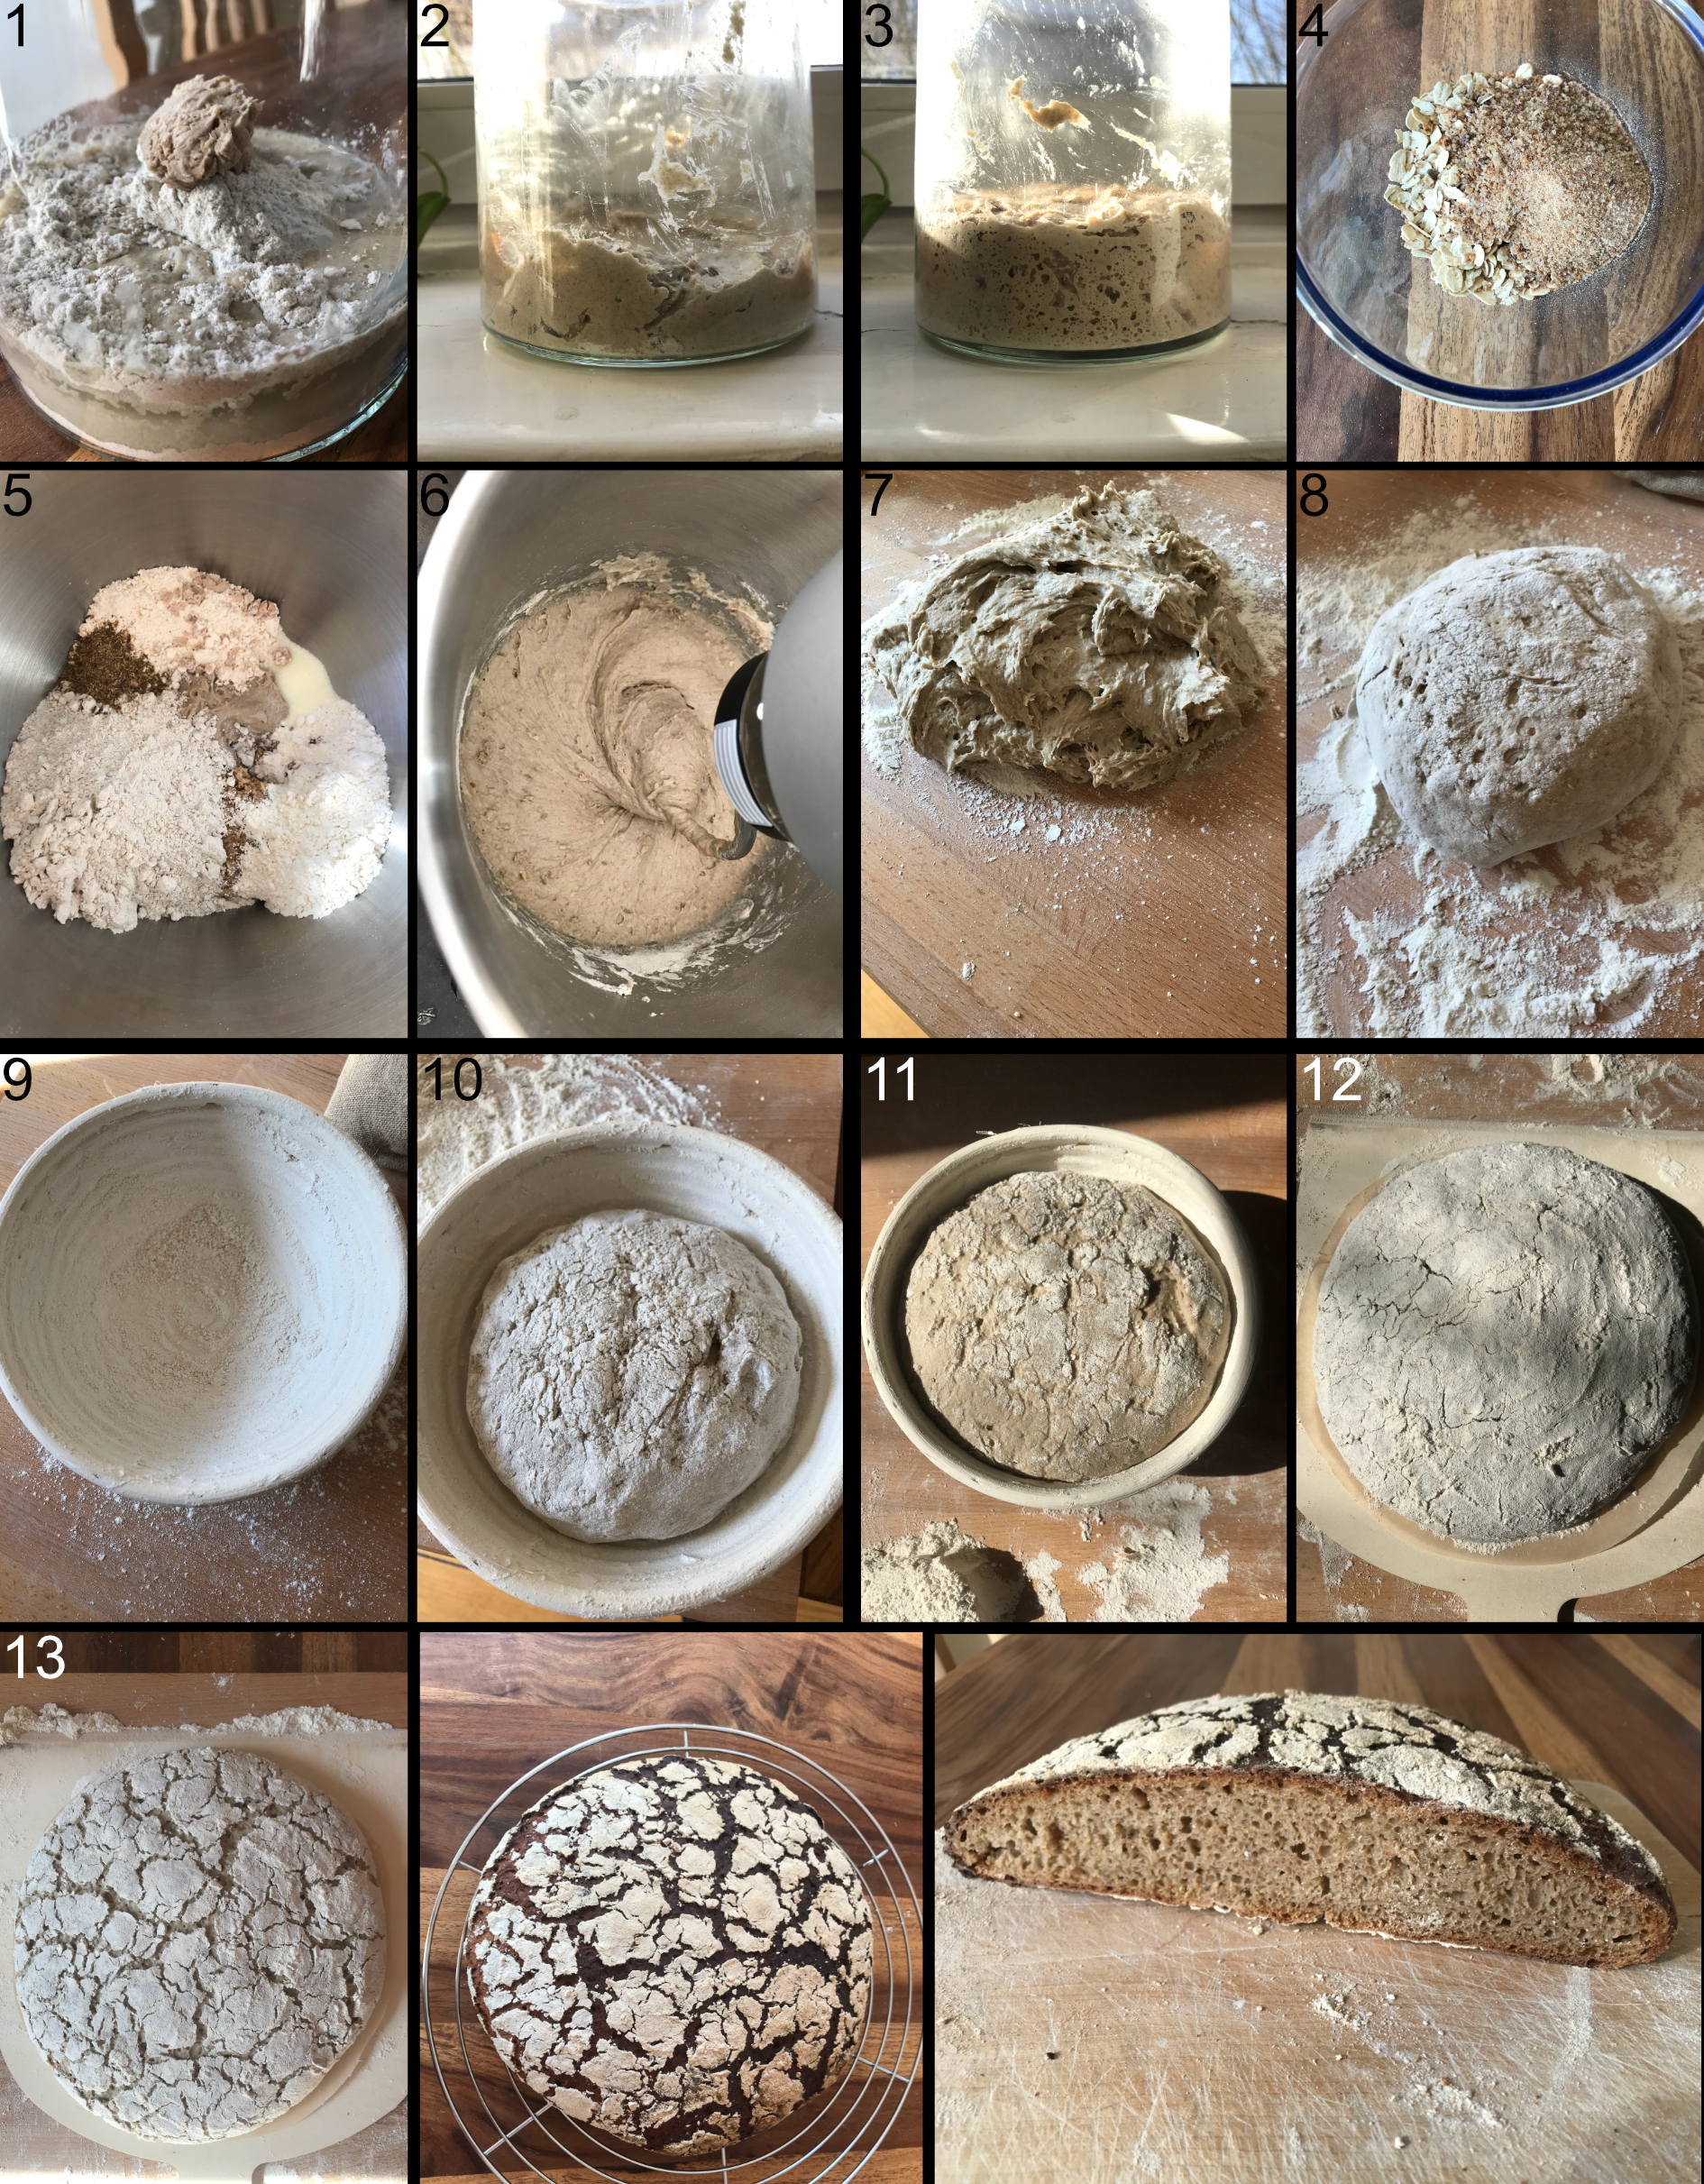
\includegraphics[width=16cm]{Pictures/Main/Bread/sourdough_bread/sourdough_bread.jpg}
    \caption[Sourdough bread]{Sourdough bread}
    \label{fig:reibeplaetzchen}
    \end{center}
\end{figure}